\documentclass[doc,12pt]{apa}        % use: 'man' for submission type; 'jou' for
                                % journal type, and 'doc' for typical latex
                                % but with figures inline with text
\usepackage{geometry} 
%\geometry{a4paper} 
\usepackage[parfill]{parskip}   % paragraphs delimited by an empty line

\usepackage{graphicx} 
\usepackage{amssymb}            % no idea what this does...
\usepackage{epstopdf}           % no idea what this does...
%\usepackage{gensymb}            % no idea what this does...

\usepackage{setspace}

\DeclareGraphicsRule{.tif}{png}{.png}{`convert #1 `dirname #1`/`basename #1 .tif`.png} \setcounter{secnumdepth}{0}  % no idea what this does...

\usepackage{apacite}
%%%%%%%%% END HEADER %%%%%%%%%

\title{Rewards are categories.} 
\author{Erik J. Peterson} \affiliation{Dept. of Psychology \\ Colorado State University \\ Fort Collins, CO} 

%%%%%%%%%%%%%%%%
\begin{document} 
%%%%%%%%%%%%%%%%
\maketitle
\doublespacing

\section{Chapter 3 -- fMRI analyses} % (fold)
\label{sec:task_and_models}
\subsection{In acquisition}
\label{sub:acquired}
fMRI data was acquired at the Intermountain Neuroimaging Consortium (INC) facility located at the University of Colorado at Boulder.  All 18 right-handed participants were be pre-screened for the typical fMRI exclusion factors (e.g. metal implants, mental disorders, etc).  Two sets of high resolution anatomical data were acquired. \emph{TODO rest of scan details, cover both localizers and ana}

Following DICOM to nifiti-1 (4D) conversion using dicom2nii (\url{http://www.mccauslandcenter.sc.edu/mricro/mricron/dcm2nii.html}), each dataset was then subjected to the following preprocessing pipeline, carried out in SPM8 using that program's batch mode (\url{http://www.fil.ion.ucl.ac.uk/spm/software/spm8/}).  For complete code see, \url{https://github.com/andsoandso/fmri/tree/master/catreward/spm\_m}).  Anatomical data (MPRAGE) was first segmented in white and grey matter regions \cite{Collignon:1995p9347}.  Based on these segments, parameters necessary for normalization into T1 MNI-352 (1 $mm$) space were calculated.  Anatomical data was then resampled from 1.27 to 1.00 $mm^3$ using fourth degree $\beta$-splines and finally normalized into MNI space.  Normalization had two steps.  The first is a Bayesian 12-parameter affine transformation \cite{Ashburner:1997p9348}.  The second is a set of nonlinear deformations, using a 1127 parameter discrete cosine transform \cite{Ashburner:1999p9350}. 

Movement regressors for all functional volumes were calculated.  No participant moved more than 1.5 $mm$. Functional data was then slice-time corrected, using slice 13 (the middle slice from the descending acquisition) as the reference. Data was then coregistered with the pre-processed (native-space) anatomical data \cite{Collignon:1995p9347}, resampled to 3 $mm^3$ again using fourth degree $\beta$-splines, and normalized into MNI space using the anatomically-derived parameters above.  Finally, the functional data was spatially smoothed using a 6 $mm$ FWHM Gaussian, though a copy of the un-smoothed data was retained for the ROI analyses.  Each voxel's timecourse was also low-pass filtered (using finite impulse response model, with a cutoff at 0.008 Hz, \cite{Kruggel:1999p9351}) prior to regression analysis.  For all whole-brain analyses, the movement regressors were entered into every model as covariates, accounting for any head movement.

All statistical parametric maps presented below were derived from a Random Effects (RFX, or ``second-level'' in SPM8 jargon) analysis, multiple comparison corrected assuming a Gaussian Random Field using the Family Wise Error Rate (FWE) at the $p < 0.05$ \cite{Worsley:1996p9367}, and a minimum cluster size of 4 voxels), that is except for the raw, unthresholded, maps of $t$-values discussed in the next section.

In fMRI (and in time-series analysis in general) there is an intrinsic trade-off between simply detecting a signal in the presence of noise and then estimating the timecourse (i.e. shape) of that signal \cite{Dale:1999p7901,Birn:2002p1777,Liu:2004p2141}.   One way to optimize over both these objectives is to manipulate the trial order, inside a rapid event-related design \cite{Miezin:2000p7924}.  One state of the art method for setting the trial order is a genetic algorithm which uses two (wieghted) loss functions, one for signal detection and one for time-course estimation \cite{Wager:2003p2980}. \citeNP{Kao:2009p7899}, improved on this design, adding in psychological considerations, and greatly improving executation speed and documentation.  As a result, Kao's method was used to optimize trial orders for part 1 and 2, along with the reward category (i.e. grating only) localizer scan.

\subsection{Maps of blobs}
\label{sub:blob}
Whole brain activity for the stimulus-response learning portion of the behavioral experiment (i.e. part 2) was examined first by comparing all trials to the baseline (rest) condition.  This data is presented in two ways.  First is a transparent overlay of the raw $t$-values.  Second is the more typical statistically thresholded contrast image.  The contrast map showed significant ($t$(15) = 6.59, $p< 0.05$) bilateral activity in the cerebellum, insula and anterior cingulate (Figure~\ref{fig:gl}).  Examination of the raw $t$-values confirms that observed significant effects were robust and widespread in their respective regions, but also allows for the analysis of overall and subthreshold patterns of activity.  These raw data suggest near threshold levels of activity in the head of the caudate, ventrol-medial, dorsal lateral frontal cortices as well as (weaker) activity in the occipital lobe (Figure~\ref{fig:raw}).  And indeed in a two-way ANOVA looking for at that interaction between gains and losses significance clusters were observed in head and body of caudate, insula, posterior and anterior cingulate with the posterior activation extending into the precuneus, dorsal lateral (i.e middle frontal) and ventral medial cortex (Figure~\ref{fig:gxl}; $F$(1, 270) = 30.76, $p < 0.05$).  When trials with gains and losses were examined separately, both showed activity in the same areas as when they were combined (not shown).  Losses showed both increases and decreased of the BOLD signal compared to the rest condition, whereas gains exhibited only increases (not shown).

\begin{figure}[tp]
	\fitfigure{f_map_gl_p05}
    \centering
    \caption{Statistical parametric map for all trials in the stimulus-response learning task (i.e. part 2), compared to the rest period.  \emph{Left} is a glass brain, showing all significant clusters mapped down to 3 two dimensional representations.  \emph{Right} is a set of axial slices highlighting strong areas of activity overlaid onto the T1 MNI-352 template.  $Z$ is the height of the axial slice in MNI space.}
	\label{fig:gl}
\end{figure}

\begin{figure}[tp]
	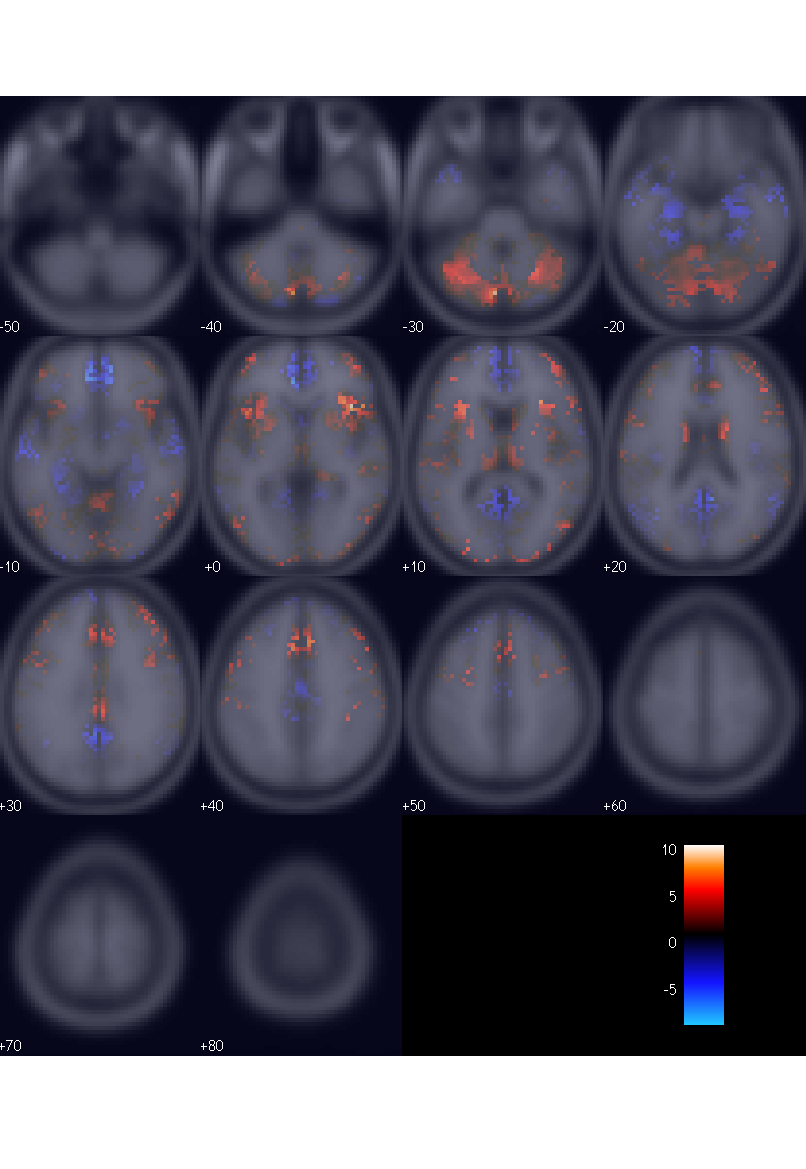
\includegraphics{f_map_gl_raw_t}
    \centering
	\caption{(Raw, that is unthresholded, $t$-values for all trials in the stimulus-response learning task (i.e. part 2), compared to the rest period,  overlaid onto the T1 MNI-352 template.   Each number is the height of the axial slice in MNI space.}
	\label{fig:glraw}
\end{figure}

\begin{figure}[tp]
	\fitfigure{f_map_gxl_p05}
    \centering
	\caption{Statistical parametric map for all trials in the stimulus-response learning task (i.e. part 2) examining the interaction between gains and losses.  \emph{Left} is a glass brain, showing all significant clusters mapped down to 3 two dimensional representations.  \emph{Right} is a set of axial slices highlighting strong areas of activity overlaid onto the T1 MNI-352 template.  $Z$ is the height of the axial slice in MNI space.}
	\label{fig:gxl}
\end{figure}

\subsection{Regions and models}
\label{sub:regoins}
\subsubsection{The right chunks}
\label{sub:chunks}
Following whole-brain analysis, regions of interest were selected.  Two methods for creating regions of interest were initially compared.  The first employed only regions from the Harvard-Oxford probabilistic anatomical atlas \cite{Desikan:2006p9370}, using the 50\% cutoff.  The second combined anatomical regions with functional clusters isolated using both data collected during the second half of part 1 of the behavioral training, and from the reward-category localizer outlined above.  Initial analyses showed that the clustered regions and entire anatomical regions model-fits were very similar.  So functional analyses were dropped.  Only anatomical based analyses are presented here.  Anatomical regions of interest were selected \emph{a priori} based on previous studies of reinforcement and category learning.  Subcortical regions of interest were the right and left dorsal caudate, putamen, ventral striatum/nucleus accumbens, hippocampus, and amygdala.   Bilateral cortical areas were the middle frontal cortex (i.e. dorsal lateral PFC), superior frontal cortex (which contains ventral medial PFC), orbital frontal cortex, anterior and posterior cingulate.

\subsubsection{Aggregating each area}
\label{sub:aggregating}
Using the nibabel library (v1.2.0; \url{http://nipy.org/nibabel}) to read the nifiti-1 files, and and Numpy (v1.6.1; \url{http://numpy.scipy.org/}) custom Python (v2.7.2) code was written that extracts the average timecourse for every

\newpage
\bibliography{bibmin}
%%%%%%%%%%%%%
\end{document}
%%%%%%%%%%%%%
